\chapter{System evaluation}
\label{System_evaluation}
The system will be evaluated on three different criteria: Precision, recall and and response time.

Precision is defined in equation \ref{eq:precsion/recall} and gives us insight in how many situations the light would turn on unnecessarily.

recall is defined in equation \ref{eq:precsion/recall} and gives us insight in how often the light fails to turns on when an object passes by. 

\begin{equation}
\label{eq:precsion/recall}
Precision = \frac{TP}{TP + FP}
\quad
Recall = \frac{TP}{TP + FN}
\end{equation}

The precise repose time is impossible to determine with the used dataset, as the starting time of the event is not defined exactly. It is however possible that if two different algorithms trigger a detection, we compare the detection times, and compare those.

\section{Hallway Evaluation}

\subsection{Test set-up}
The system was evaluated indoor and outdoor. 

\begin{figure}
	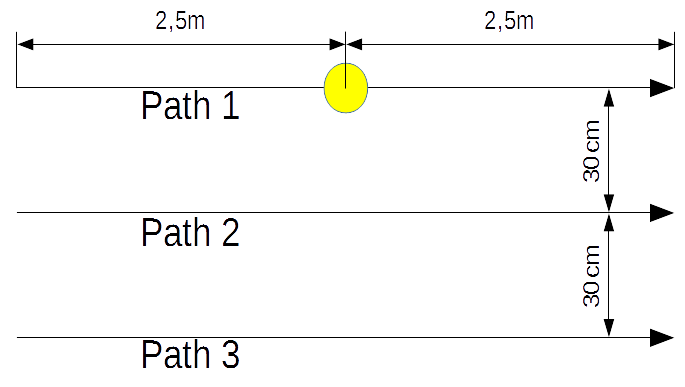
\includegraphics[width=\textwidth]{pics/Evaluation_paths.png}
	\caption{The three paths the test subjects had to walk underneath the light.}
	\label{fig:Evaluation_paths}
\end{figure}

\begin{figure}
	\centering     %%% not \center
	\label{fig:TestPicture}
	\subfigure[Indoor]{\label{fig:setup_a}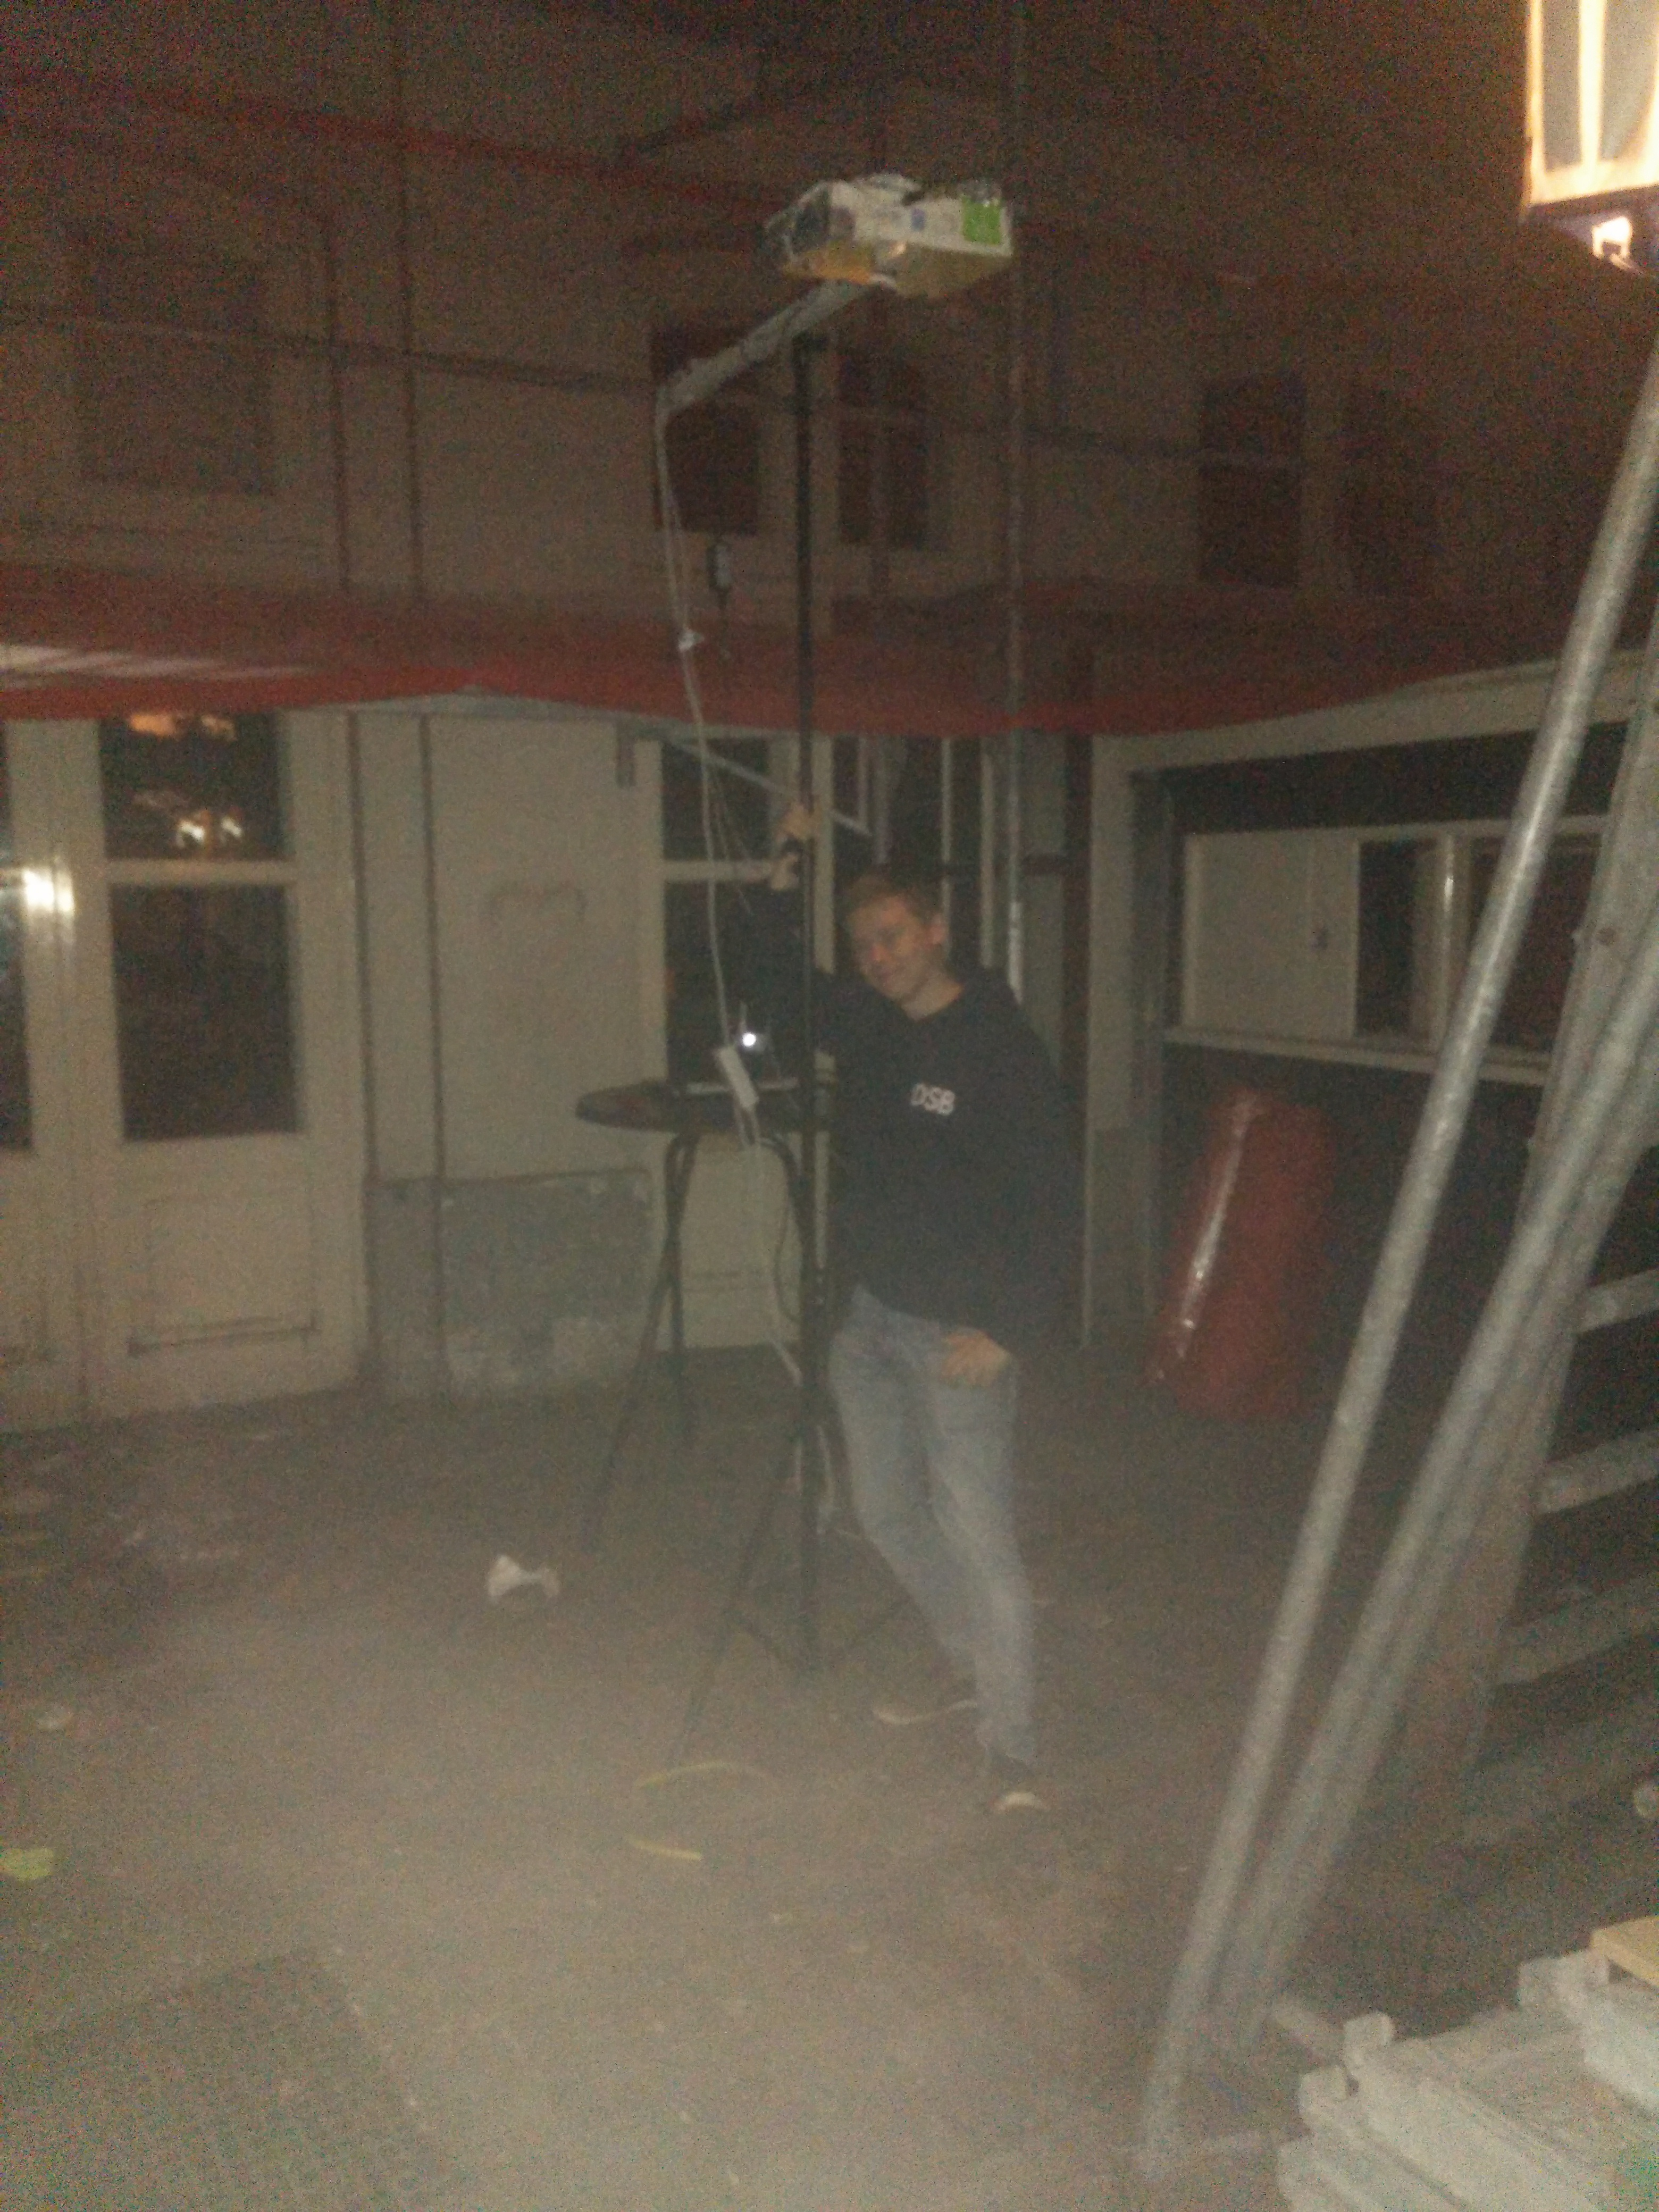
\includegraphics[width=60mm]{pics/Setup_outdoor.jpg}}
	\subfigure[Outdoor]{\label{fig:setup_b}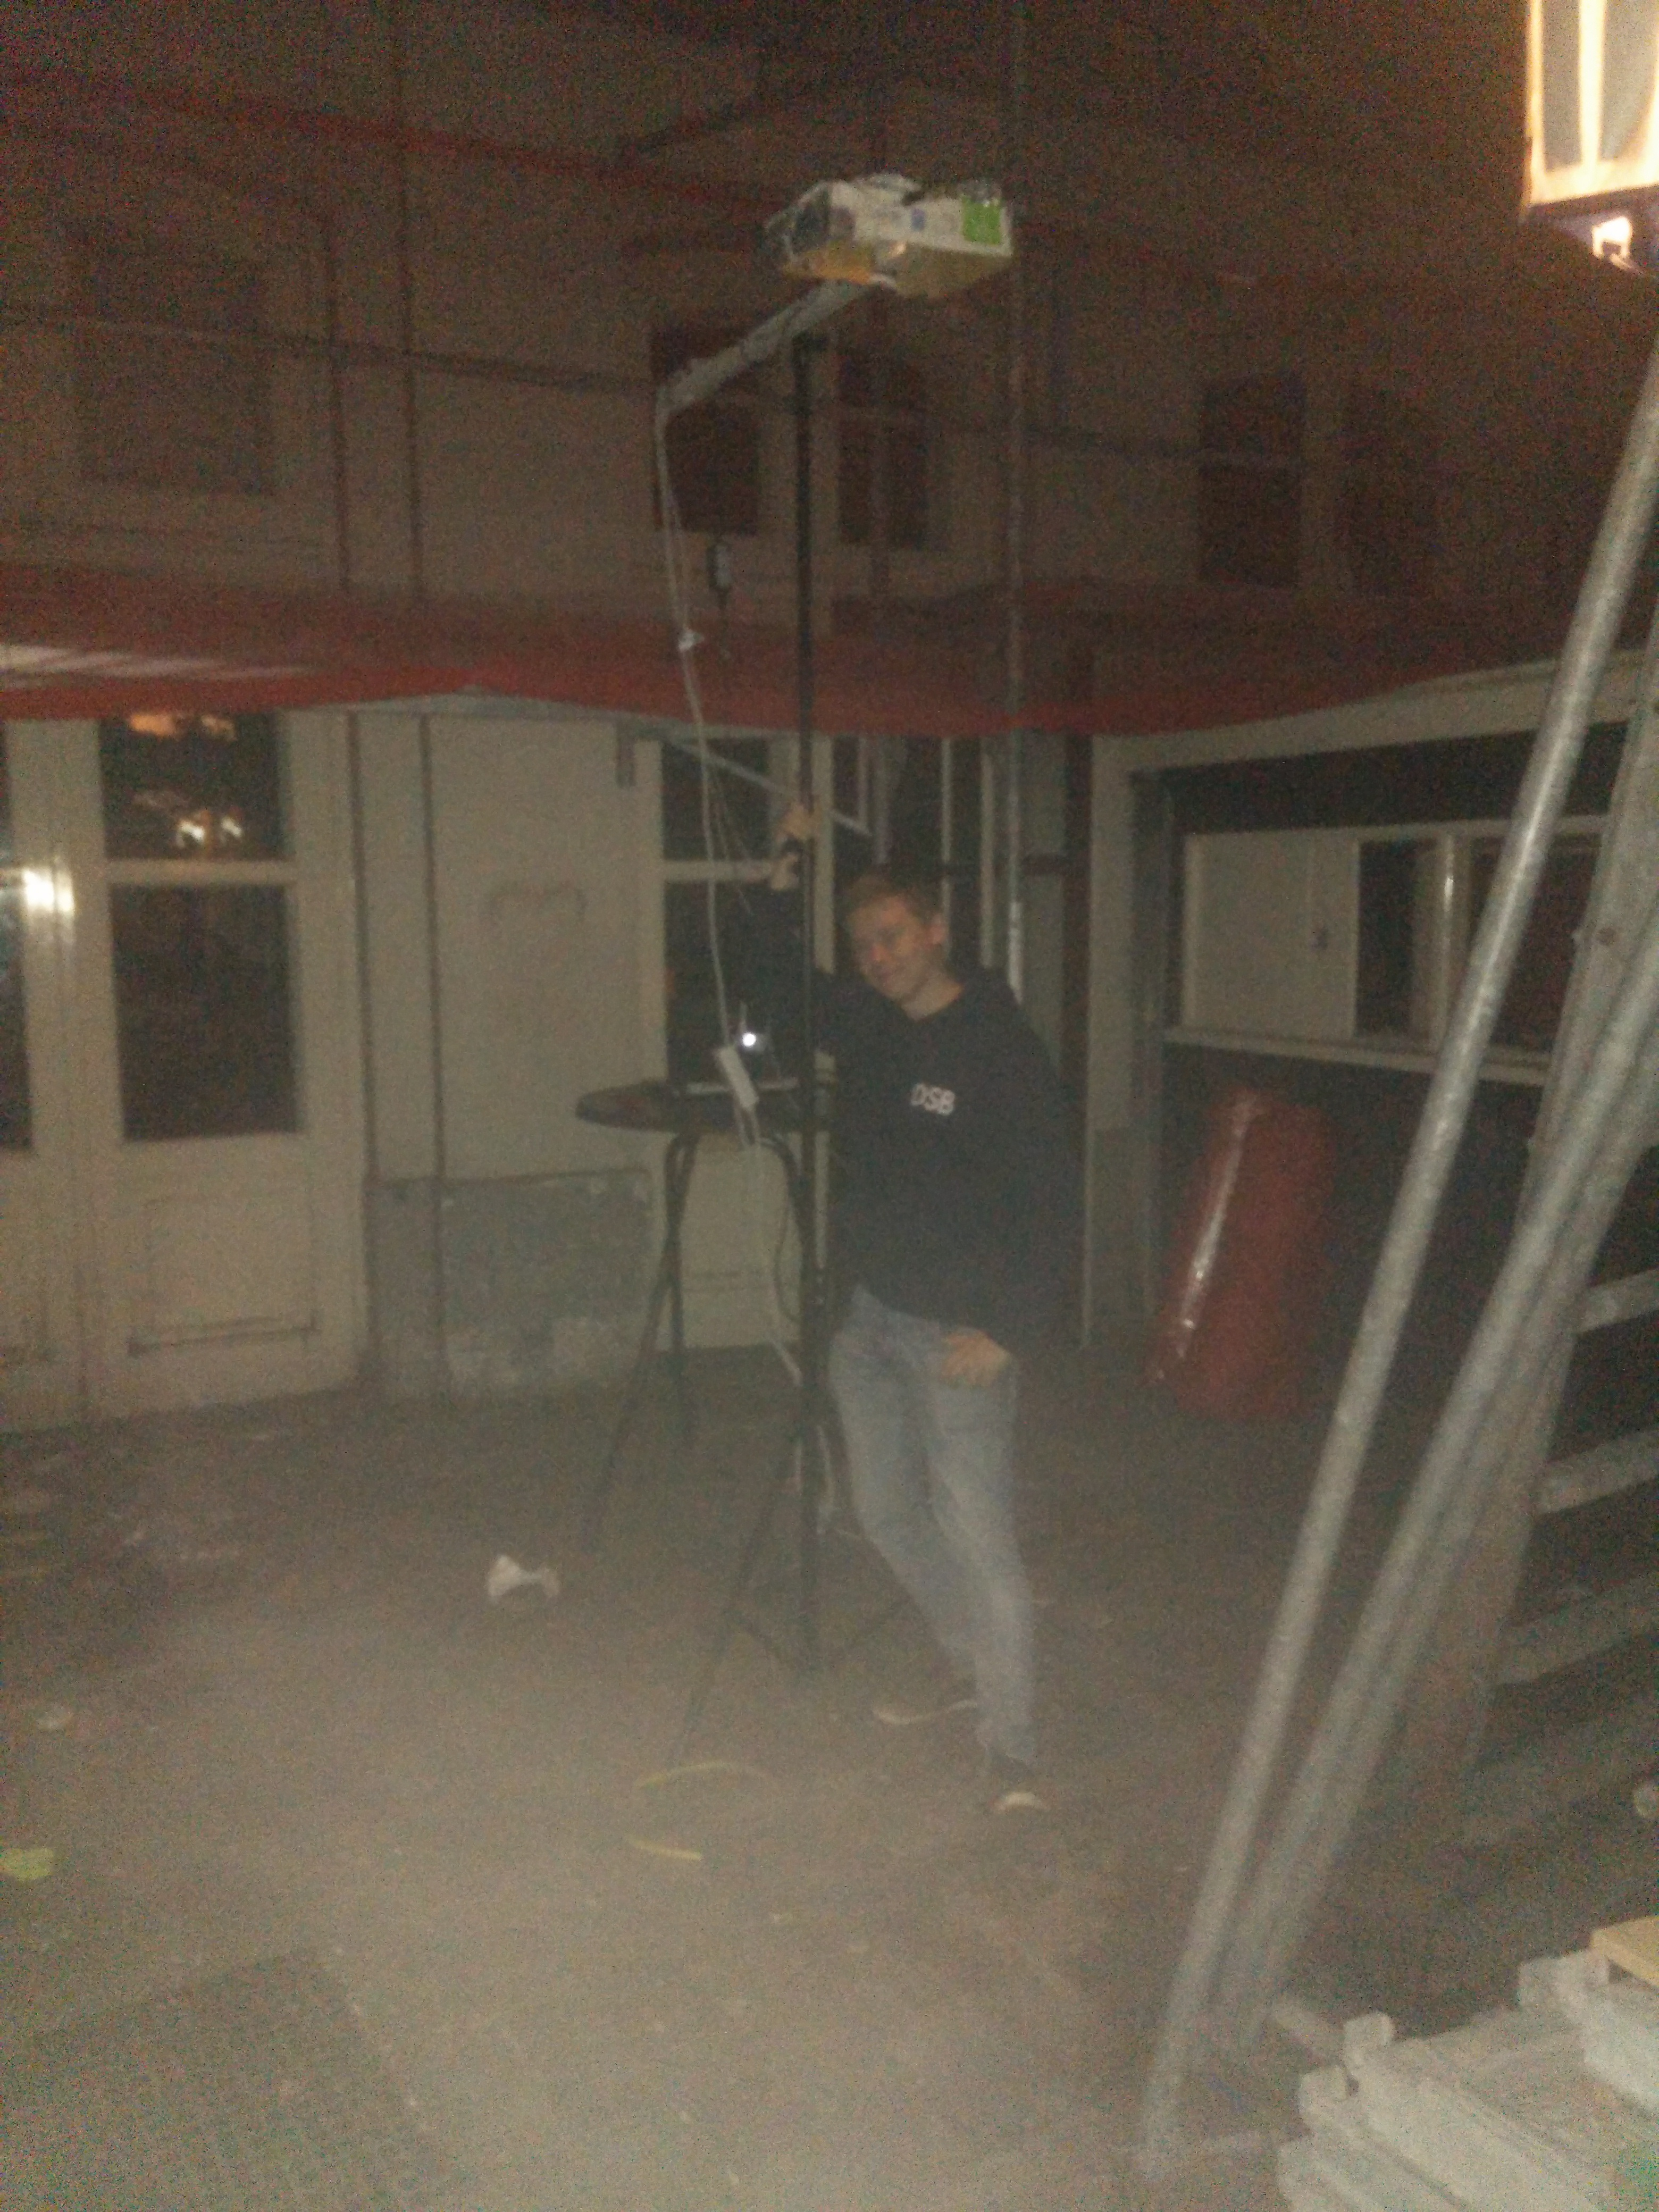
\includegraphics[width=60mm]{pics/Setup_outdoor.jpg}}
	\caption{Pictures of the test setup indoor (a) and outdoor (b). The light was suspended at 2.6m high.}
\end{figure}

\subsection{indoor results}

\subsection{outdoor results}

\section{Street}

\subsection{Test set-up}